% ============================================================
% HPTU Nueva Sede — Segunda Reunión de Avance
% Presentación narrativa: avances vs reunión anterior
% Compilar con: lualatex hptu-avance-2.tex
% ============================================================
\documentclass[aspectratio=169, 11pt]{beamer}

% ── Tema y colores ──────────────────────────────────────────
\usetheme{default}
\usecolortheme{default}
\setbeamertemplate{navigation symbols}{}
\setbeamertemplate{footline}[frame number]

% Paleta HPTU
\definecolor{hptu}{HTML}{00549F}
\definecolor{hptudark}{HTML}{003D75}
\definecolor{teal}{HTML}{0D9488}
\definecolor{coral}{HTML}{EF4444}
\definecolor{amber}{HTML}{F59E0B}
\definecolor{slate}{HTML}{64748B}
\definecolor{bglight}{HTML}{F8FAFC}
\definecolor{green}{HTML}{22C55E}

\setbeamercolor{frametitle}{fg=hptu}
\setbeamercolor{title}{fg=white}
\setbeamercolor{subtitle}{fg=white!85}
\setbeamercolor{author}{fg=white!80}
\setbeamercolor{date}{fg=white!70}
\setbeamercolor{normal text}{fg=black!85}
\setbeamercolor{structure}{fg=hptu}
\setbeamercolor{itemize item}{fg=teal}
\setbeamercolor{itemize subitem}{fg=hptu}
\setbeamercolor{block title}{fg=white, bg=hptu}
\setbeamercolor{block body}{bg=bglight}
\setbeamercolor{block title alerted}{fg=white, bg=coral}
\setbeamercolor{block body alerted}{bg=coral!5}
\setbeamercolor{block title example}{fg=white, bg=teal}
\setbeamercolor{block body example}{bg=teal!5}

\setbeamerfont{frametitle}{size=\Large, series=\bfseries}
\setbeamerfont{title}{size=\Huge, series=\bfseries}
\setbeamerfont{subtitle}{size=\large}
\setbeamertemplate{itemize items}[circle]

% ── Paquetes ────────────────────────────────────────────────
\usepackage{fontspec}
\usepackage{booktabs}
\usepackage{tabularx}
\usepackage{colortbl}
\usepackage{graphicx}
\usepackage{tikz}
\usetikzlibrary{calc, positioning, shapes.geometric, arrows.meta, backgrounds}
\usepackage{pgfplots}
\pgfplotsset{compat=1.18}
\usepackage{multicol}
\usepackage{hyperref}
\usepackage{soul}

% Fuentes
\setsansfont{Helvetica Neue}[
  BoldFont={Helvetica Neue Bold},
  ItalicFont={Helvetica Neue Italic},
]

\newcommand{\highlight}[1]{\textcolor{teal}{\textbf{#1}}}
\newcommand{\danger}[1]{\textcolor{coral}{\textbf{#1}}}
\newcommand{\src}[1]{\par\vspace{2pt}{\tiny\textcolor{slate}{Fuente: #1}}}
\newcommand{\antes}[1]{\textcolor{slate}{\sout{#1}}}
\newcommand{\ahora}[1]{\textcolor{teal}{\textbf{#1}}}

% ── Metadata ────────────────────────────────────────────────
\title{Estudio de Localización\\Estratégica}
\subtitle{HPTU Nueva Sede — Segunda Reunión de Avance}
\author{Equipo de Análisis Estratégico}
\date{4 de marzo, 2026}

\begin{document}

% ============================================================
% PORTADA
% ============================================================
{
\setbeamercolor{background canvas}{bg=hptu}
\begin{frame}[plain]
\vfill
\begin{center}
{\usebeamerfont{title}\usebeamercolor[fg]{title}\inserttitle}

\vspace{8pt}
{\usebeamerfont{subtitle}\usebeamercolor[fg]{subtitle}\insertsubtitle}

\vspace{20pt}
\begin{tikzpicture}
  \draw[white, line width=0.5pt] (0,0) -- (6,0);
\end{tikzpicture}

\vspace{12pt}
{\small\usebeamercolor[fg]{date}
De 9 a 12 capas $\cdot$ 145 IPS mapeadas $\cdot$ Modelo financiero preliminar}

\vspace{20pt}
{\footnotesize\usebeamercolor[fg]{author}\insertdate}
\end{center}
\vfill
\end{frame}
}

% ============================================================
% AGENDA
% ============================================================
\begin{frame}{¿Qué veremos hoy?}

En la reunión anterior presentamos las \textbf{Fases 1 y 2}: demanda, flujos, scoring MCDA.

\vspace{8pt}
Hoy mostramos \textbf{qué hicimos después} de esa reunión:

\vspace{12pt}
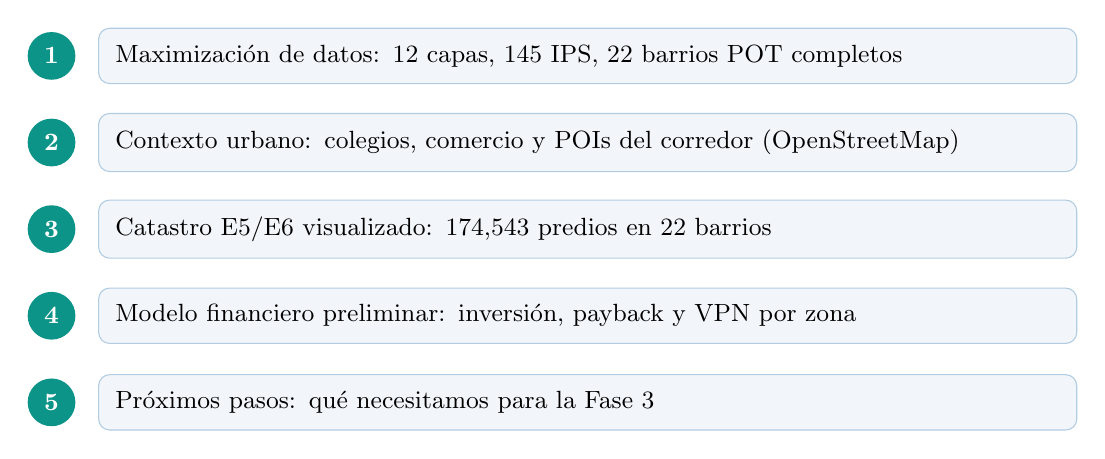
\begin{tikzpicture}[
  item/.style={draw=hptu!30, fill=hptu!5, rounded corners=4pt,
               text width=12cm, minimum height=0.7cm, align=left,
               font=\small, inner sep=6pt},
  num/.style={circle, fill=teal, text=white, font=\small\bfseries, minimum size=0.6cm}
]
\node[item] (a) at (0,0) {Maximización de datos: 12 capas, 145 IPS, 22 barrios POT completos};
\node[num, left=8pt of a] {1};

\node[item] (b) at (0,-1.1) {Contexto urbano: colegios, comercio y POIs del corredor (OpenStreetMap)};
\node[num, left=8pt of b] {2};

\node[item] (c) at (0,-2.2) {Catastro E5/E6 visualizado: 174,543 predios en 22 barrios};
\node[num, left=8pt of c] {3};

\node[item] (d) at (0,-3.3) {Modelo financiero preliminar: inversión, payback y VPN por zona};
\node[num, left=8pt of d] {4};

\node[item] (e) at (0,-4.4) {Próximos pasos: qué necesitamos para la Fase 3};
\node[num, left=8pt of e] {5};
\end{tikzpicture}

\vspace{8pt}
{\small\textcolor{slate}{Todo está en la plataforma: \url{https://hptu-localizacion.vercel.app}}}
\end{frame}

% ============================================================
% ANTES VS AHORA — RESUMEN
% ============================================================
{
\setbeamercolor{background canvas}{bg=hptu!3}
\begin{frame}{Antes vs.\ ahora: el mapa creció}

\begin{center}
\large ¿Qué cambió desde la reunión anterior?
\end{center}

\vspace{10pt}
\begin{center}
{\small
\begin{tabular}{@{}l c c l@{}}
\toprule
\textbf{Métrica} & \textbf{Reunión 1} & \textbf{Hoy} & \textbf{Cambio} \\
\midrule
Capas en el mapa & 9 & \highlight{12} & +3 nuevas \\
IPS mostradas & 34 & \highlight{145} & +111 (\textbf{4.3$\times$}) \\
Barrios POT & 15 & \highlight{22} & +7 (ahora \textbf{completo}) \\
POIs corredor (OSM) & 0 & \highlight{63} & Colegios, comercio, salud \\
Catastro burbujas & solo datos & \highlight{22 barrios} & Visualización interactiva \\
Modelo financiero & ninguno & \highlight{5 zonas} & VPN, payback, inversión \\
Sección web financiera & no existía & \highlight{Dashboard} & Con supuestos trazables \\
\midrule
\textbf{Datos procesados} & \textbf{3.8M} & \textbf{3.8M+} & Mismos datos, más visibles \\
\bottomrule
\end{tabular}
}
\end{center}

\vspace{10pt}
\begin{exampleblock}{\small La filosofía}
\small No recolectamos más datos --- \textbf{visualizamos todo} lo que ya teníamos. La reunión anterior mostraba el 5\% de los datos procesados. Hoy mostramos significativamente más.
\end{exampleblock}
\end{frame}
}

% ============================================================
% RED DE SALUD COMPLETA
% ============================================================
\begin{frame}{La red de salud: ahora vemos las 145 IPS}

\begin{columns}[T]
\column{0.55\textwidth}
Antes mostrábamos \textbf{34 puntos} (solo alta complejidad).\\
Ahora mostramos \textbf{toda la red}:

\vspace{8pt}
{\small
\begin{tabular}{@{}lccc@{}}
\toprule
\textbf{Complejidad} & \textbf{IPS} & \textbf{Color} & \textbf{Radio} \\
\midrule
\rowcolor{coral!8}
Alta & 25 & \danger{Rojo} & Grande \\
Mediana & 48 & \textcolor{amber}{Naranja} & Mediano \\
Baja / Consulta & 72 & Gris & Pequeño \\
\midrule
\textbf{Total} & \textbf{145} & & \\
\bottomrule
\end{tabular}
}

\vspace{8pt}
Cada punto tiene \textbf{popup interactivo} con:
\begin{itemize}\small
  \item Nombre, complejidad y naturaleza
  \item Número de camas (si aplica)
  \item ESE o privada
  \item Distancia a zona candidata más cercana
\end{itemize}

\column{0.42\textwidth}
\begin{alertblock}{\small ¿Por qué importa?}
\footnotesize Con 34 puntos veíamos dónde compiten los grandes.\\
Con 145 vemos \textbf{el ecosistema completo}: dónde hay consultorios (referidores), y dónde hay vacíos.
\end{alertblock}

\vspace{4pt}
\begin{block}{\small Hallazgo clave}
\footnotesize Las 145 IPS se \textbf{agrupan} en El Poblado centro y Envigado.\\[3pt]
El corredor Las Palmas tiene \danger{densidad casi nula} --- ni siquiera consultorios.\\[3pt]
No solo faltan camas de alta complejidad, falta \textbf{toda la cadena}.
\end{block}
\end{columns}
\end{frame}

% ============================================================
% CATASTRO E5/E6 VISUALIZADO
% ============================================================
\begin{frame}{Catastro E5/E6: el mercado objetivo, barrio por barrio}

\begin{columns}[T]
\column{0.52\textwidth}
1.04M predios ahora como \textbf{burbujas proporcionales} por barrio:

\vspace{4pt}
{\scriptsize
\begin{tabular}{@{}lrrl@{}}
\toprule
\textbf{Barrio} & \textbf{E5+E6} & \textbf{\%} & \textbf{Avalúo} \\
\midrule
\rowcolor{teal!10}
\textbf{El Poblado} & \textbf{38,415} & \textbf{98\%} & \$371M \\
Castropol & 6,228 & 97\% & \$327M \\
Los Balsos No.\ 1 & 4,019 & 95\% & \$401M \\
San Lucas & 3,671 & 93\% & \$512M \\
\rowcolor{teal!6}
Altos del Poblado & 1,867 & 91\% & \$245M \\
El Tesoro & 1,856 & 89\% & \$258M \\
Los Balsos No.\ 2 & 2,143 & 88\% & \$347M \\
\midrule
\textbf{22 barrios} & \textbf{174,543} & & \\
\bottomrule
\end{tabular}
}

\src{Catastro Municipal Medellín (bp59-rj8r), 1,041,413 predios}

\column{0.45\textwidth}
\vspace{4pt}
\begin{exampleblock}{\small ¿Qué dicen las burbujas?}
\footnotesize
\textbf{Tamaño} = predios E5/E6. \textbf{Color} = \% concentración.\\
Click = avalúo promedio, totales, estrato.
\end{exampleblock}

\vspace{4pt}
\begin{block}{\small Insight}
\footnotesize El Poblado core tiene 38K predios. Pero los barrios del corredor (Altos del Poblado, El Tesoro, Los Balsos) tienen \textbf{91-95\%} E5/E6 con avalúos de \highlight{\$245M--\$512M COP}.\\[3pt]
\textbf{Alta capacidad de pago} y \textbf{cero infraestructura hospitalaria}.
\end{block}
\end{columns}
\end{frame}

% ============================================================
% POT COMPLETO — 22 BARRIOS
% ============================================================
\begin{frame}{POT: ahora con los 22 barrios completos}

\begin{columns}[T]
\column{0.55\textwidth}
Antes: 15 barrios. Ahora: \textbf{22 barrios} clasificados por viabilidad:

\vspace{6pt}
\begin{center}
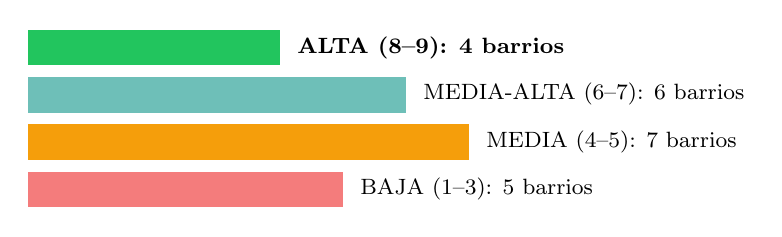
\begin{tikzpicture}
  \fill[green] (0,0) rectangle (4*0.8, 0.45);
  \node[right, font=\footnotesize\bfseries] at (4*0.8+0.1, 0.22) {ALTA (8--9): 4 barrios};
  \fill[teal!60] (0,-0.6) rectangle (6*0.8, -0.15);
  \node[right, font=\footnotesize] at (6*0.8+0.1, -0.37) {MEDIA-ALTA (6--7): 6 barrios};
  \fill[amber] (0,-1.2) rectangle (7*0.8, -0.75);
  \node[right, font=\footnotesize] at (7*0.8+0.1, -0.97) {MEDIA (4--5): 7 barrios};
  \fill[coral!70] (0,-1.8) rectangle (5*0.8, -1.35);
  \node[right, font=\footnotesize] at (5*0.8+0.1, -1.57) {BAJA (1--3): 5 barrios};
\end{tikzpicture}
\end{center}

\vspace{4pt}
{\scriptsize Cada punto: CL\_D, ICS, ICF, suelo potencial (m²), altura máxima (pisos).}

\column{0.42\textwidth}
\begin{exampleblock}{\small Top 4: viabilidad ALTA}
\footnotesize
\begin{tabular}{@{}lcc@{}}
\toprule
\textbf{Barrio} & \textbf{Score} & \textbf{CL\_D} \\
\midrule
\rowcolor{teal!10}
Altos del Poblado & \highlight{9/9} & 2.38 \\
El Tesoro & 9/9 & 2.52 \\
Castropol & 8/9 & 1.89 \\
Los Balsos No.\ 1 & 8/9 & 2.15 \\
\bottomrule
\end{tabular}
\end{exampleblock}

\vspace{4pt}
\begin{alertblock}{\small 7 barrios nuevos}
\footnotesize Patio Bonito, El Diamante, Villa Carlota y otros --- todos con score \textbf{MEDIA o BAJA}. Confirma que las mejores zonas son las ya identificadas.
\end{alertblock}
\end{columns}
\end{frame}

% ============================================================
% CONTEXTO URBANO — POIs OSM
% ============================================================
\begin{frame}{Contexto urbano: colegios, comercio y servicios}

\begin{columns}[T]
\column{0.55\textwidth}
\textbf{63 POIs} de OpenStreetMap integrados al corredor:

\vspace{6pt}
{\footnotesize
\begin{tabular}{@{}lrll@{}}
\toprule
\textbf{Categoría} & \textbf{POIs} & \textbf{Color} & \textbf{Ejemplos} \\
\midrule
Educación & 30 & \textcolor{violet}{\textbf{Morado}} & Marymount, Columbus, EIA \\
Comercio & 28 & \textcolor{amber}{\textbf{Ámbar}} & CC El Tesoro, Oviedo \\
Salud & 5 & \textcolor{coral}{\textbf{Rojo}} & Clínicas menores \\
\midrule
\textbf{Total} & \textbf{63} & & \\
\bottomrule
\end{tabular}
}

\vspace{4pt}
{\scriptsize Popup con nombre, categoría y distancia a zona candidata.}
\src{OpenStreetMap Overpass API, 1,323 POIs descargados, 63 en corredor}

\column{0.42\textwidth}
\begin{block}{\small ¿Por qué importa?}
\footnotesize Los colegios generan \textbf{tráfico cautivo} de familias E5/E6 que pasan por la zona \textbf{2 veces/día}: alta capacidad de pago, prepagada/póliza, necesitan acceso rápido a urgencias.
\end{block}

\vspace{4pt}
\begin{exampleblock}{\small Dato clave}
\footnotesize El segmento de colegios (Columbus, Marymount, Carabobo) coincide con el \danger{cuello de botella} (13.4 km/h).\\[3pt]
Un hospital \textbf{después} de esa zona captura ese flujo sin la congestión.
\end{exampleblock}
\end{columns}
\end{frame}

% ============================================================
% MODELO FINANCIERO — INTRODUCCIÓN
% ============================================================
\begin{frame}{Modelo financiero: ¿cuánto cuesta y cuándo se recupera?}

{\footnotesize Modelo \textbf{preliminar}. Cifras con {\textcolor{coral}{$\blacktriangledown$}} requieren validación.}

\vspace{4pt}
\begin{columns}[T]
\column{0.55\textwidth}

{\footnotesize
\begin{tabular}{@{}l r r r r@{}}
\toprule
\textbf{Zona} & \textbf{Camas} & \textbf{Inversión} & \textbf{Payback} & \textbf{VPN 10y} \\
\midrule
\rowcolor{teal!10}
\textbf{Las Palmas Bajo} & \textbf{250} & \textbf{\$90MM} & \textbf{11.3y} & \highlight{+\$4.8MM} \\
Las Palmas Medio & 300 & \$108MM & 9.4y & +\$15.3MM \\
Envigado--Zúñiga & 220 & \$82MM & 11.3y & +\$4.0MM \\
Nuevo Poblado & 260 & \$98MM & 9.6y & +\$14.7MM \\
\rowcolor{coral!8}
Las Palmas Alto & 150 & \$55MM & \danger{22.9y} & \danger{--\$31MM} \\
\bottomrule
\end{tabular}
}

\vspace{3pt}
{\tiny Cifras en miles de millones COP. WACC 12\%, ramp-up 60\%/80\%/100\% años 1/2/3+.}

\vspace{6pt}
{\scriptsize\textbf{Parámetros base:}
Construcción \$4.0M/m² (Scielo) · Dotación 25\% (DNP) · Ocupación 80\% · Ingreso/cama \$1,600M (HUSI) {\textcolor{coral}{$\blacktriangledown$}} · EBITDA 8\% {\textcolor{coral}{$\blacktriangledown$}} · WACC 12\% {\textcolor{coral}{$\blacktriangledown$}}
}

\column{0.42\textwidth}
\begin{exampleblock}{\small Lectura rápida}
\footnotesize
\textbf{4 de 5 zonas} con VPN positivo. LP Bajo: \highlight{\$90MM inversión}, payback 11.3 años, VPN +\$4.8MM. LP Medio: mejor VPN (\$15.3MM) por escala.\\[3pt]
Las Palmas Alto: \danger{inviable} (payback >22y, VPN negativo).
\end{exampleblock}

\vspace{4pt}
\begin{alertblock}{\small Sensibilidad}
\footnotesize Con ingreso/cama de \$2,000M (privado premium) en vez de \$1,600M (HUSI), el VPN de LP Bajo sube a \textbf{+\$25MM}. La sensibilidad al ingreso/cama es \textbf{altísima}.
\end{alertblock}
\end{columns}
\end{frame}

% ============================================================
% MODELO FINANCIERO — DETALLE POR ZONA
% ============================================================
\begin{frame}{Estructura de inversión y hallazgo clave}

\begin{columns}[T]
\column{0.55\textwidth}

{\footnotesize
\begin{tabular}{@{}l r r r r@{}}
\toprule
\textbf{Componente} & \textbf{LP Bajo} & \textbf{LP Medio} & \textbf{Envigado} & \textbf{N. Poblado} \\
\midrule
Suelo & \$15MM & \$14MM & \$20MM & \$18MM \\
Construcción & \$60MM & \$72MM & \$56MM & \$64MM \\
Equipamiento & \$15MM & \$18MM & \$14MM & \$16MM \\
\midrule
\textbf{Total} & \textbf{\$90MM} & \textbf{\$104MM} & \textbf{\$90MM} & \textbf{\$98MM} \\
\bottomrule
\end{tabular}
}

\vspace{4pt}
{\tiny Cifras redondeadas en miles de millones COP.}

\vspace{6pt}
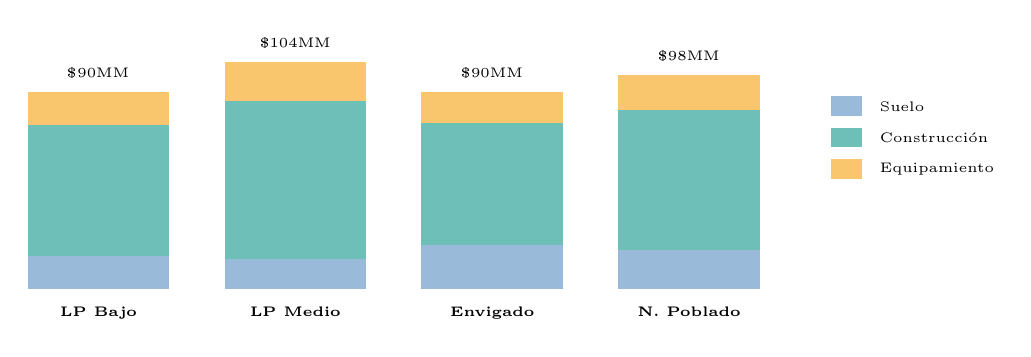
\begin{tikzpicture}
  \foreach \x/\label/\land/\const/\equip/\total in {
    0/LP Bajo/15/60/15/90,
    2.5/LP Medio/14/72/18/104,
    5/Envigado/20/56/14/90,
    7.5/N. Poblado/18/64/16/98} {
    \pgfmathsetmacro{\landh}{\land/90*2.5}
    \pgfmathsetmacro{\consth}{\const/90*2.5}
    \pgfmathsetmacro{\equiph}{\equip/90*2.5}
    \fill[hptu!40] (\x,0) rectangle (\x+1.8, \landh);
    \fill[teal!60] (\x,\landh) rectangle (\x+1.8, \landh+\consth);
    \fill[amber!60] (\x,\landh+\consth) rectangle (\x+1.8, \landh+\consth+\equiph);
    \node[font=\tiny\bfseries, below] at (\x+0.9, -0.1) {\label};
    \node[font=\tiny, above] at (\x+0.9, \landh+\consth+\equiph+0.05) {\$\total MM};
  }
  \fill[hptu!40] (10.2,2.2) rectangle (10.6,2.45); \node[font=\tiny, right] at (10.7,2.32) {Suelo};
  \fill[teal!60] (10.2,1.8) rectangle (10.6,2.05); \node[font=\tiny, right] at (10.7,1.92) {Construcción};
  \fill[amber!60] (10.2,1.4) rectangle (10.6,1.65); \node[font=\tiny, right] at (10.7,1.52) {Equipamiento};
\end{tikzpicture}

\column{0.42\textwidth}
\begin{block}{\small El suelo no es el factor decisivo}
\footnotesize El suelo = solo \textbf{15--22\%} del total.
La construcción = \textbf{67\%}.\\[3pt]
La diferencia de precio entre zonas (\$500K--\$2.5M/m²) tiene \textbf{menos impacto} del esperado.\\[3pt]
Lo que importa:
\begin{enumerate}\footnotesize
  \item Tamaño del lote disponible
  \item Altura permitida (POT)
  \item Accesibilidad (ocupación)
\end{enumerate}
\end{block}

\vspace{4pt}
\begin{exampleblock}{\small Timeline estimado}
\footnotesize
\begin{tabular}{@{}ll@{}}
Diseño + licencias & 18 meses {\textcolor{coral}{$\blacktriangledown$}} \\
Construcción & 36 meses \\
\textbf{Total} & \textbf{54 meses (4.5 años)} \\
\end{tabular}
\end{exampleblock}
\end{columns}
\end{frame}

% ============================================================
% PARÁMETROS POR VALIDAR
% ============================================================
{
\setbeamercolor{background canvas}{bg=coral!3}
\begin{frame}{Supuestos por validar: la tarea pendiente}

{\footnotesize El modelo es tan bueno como sus supuestos. Estos requieren validación:}

\vspace{4pt}
{\scriptsize
\begin{tabular}{@{}p{3.8cm}ccl@{}}
\toprule
\textbf{Parámetro} & \textbf{Prioridad} & \textbf{Valor} & \textbf{Cómo validar} \\
\midrule
\rowcolor{coral!8}
Precio suelo/m² por zona & \danger{ALTA} & \$0.5--2.5M & Lonja de Propiedad Raíz \\
\rowcolor{coral!8}
Ingreso/cama/año & \danger{ALTA} & \$1,600M & Cl.\ Pablo Tobón, Las Américas \\
\rowcolor{coral!5}
Margen EBITDA operativo & \danger{ALTA} & 8\% & Supersalud \\
Fichas normativas POT & \danger{ALTA} & Estimadas & DAP Medellín \\
Tamaño lote disponible & \danger{ALTA} & 8--15K m² & Inmobiliarias \\
\rowcolor{amber!10}
WACC del proyecto & MEDIA & 12\% & Banca de inversión \\
\rowcolor{amber!10}
Costos diseño + licencias & MEDIA & Estimados & Arq.\ hospitalaria \\
\bottomrule
\end{tabular}
}

\vspace{6pt}
\begin{columns}[T]
\column{0.48\textwidth}
\begin{alertblock}{\small Sensibilidad crítica}
\footnotesize Si ingreso/cama sube a \$2,000M (+25\%), el VPN se multiplica \textbf{3--5$\times$}. Es el parámetro más sensible.
\end{alertblock}

\column{0.48\textwidth}
\begin{block}{\small Fuentes}
\footnotesize Construcción: Scielo/U. Militar. Benchmark: HUSI 2024. Suelo: Fincaraíz, Metrocuadrado. Sector: DNP Proyectos Tipo.
\end{block}
\end{columns}
\end{frame}
}

% ============================================================
% TABLERO INTEGRAL
% ============================================================
\begin{frame}{Tablero integral: 12 capas interactivas}

\begin{columns}[T]
\column{0.48\textwidth}
{\footnotesize\textbf{Base (4):} Estratos 5/6, Corredor, HPTU, POIs clave}

\vspace{4pt}
{\footnotesize\textbf{Datos (5):}}
\begin{itemize}\scriptsize
  \item[\textcolor{amber}{$\bullet$}] Tráfico por tramo (8 segmentos)
  \item[\textcolor{coral}{$\bullet$}] \highlight{Red salud (145 IPS)} {\tiny\textcolor{teal}{NUEVO}}
  \item[\textcolor{hptu}{$\bullet$}] \highlight{Catastro E5/E6 (22 barrios)} {\tiny\textcolor{teal}{NUEVO}}
  \item[\textcolor{violet}{$\bullet$}] \highlight{Colegios corredor (30)} {\tiny\textcolor{teal}{NUEVO}}
  \item[\textcolor{amber}{$\bullet$}] \highlight{Comercio corredor (28)} {\tiny\textcolor{teal}{NUEVO}}
\end{itemize}

\vspace{2pt}
{\footnotesize\textbf{Análisis (3):}}
\begin{itemize}\scriptsize
  \item[\textcolor{green}{$\bullet$}] \highlight{Viabilidad POT (22)} {\tiny\textcolor{teal}{AMPLIADO}}
  \item[\textcolor{amber}{$\bullet$}] Isocronas (10/20/30 min)
  \item[\textcolor{hptu}{$\bullet$}] Rutas alternas (6)
\end{itemize}

\vspace{4pt}
{\footnotesize Cada capa: toggle on/off, popups al click, clustering dinámico, leyenda colapsible.}

\column{0.49\textwidth}
\begin{block}{\small Capas más relevantes para la Junta}
\footnotesize
\begin{enumerate}\footnotesize
  \item \textbf{Red de salud}: muestra el vacío en el corredor
  \item \textbf{Catastro E5/E6}: dimensiona el mercado
  \item \textbf{Viabilidad POT}: dónde se puede construir
  \item \textbf{Isocronas}: tiempos de acceso
  \item \textbf{Tráfico}: por qué Las Palmas fluye
\end{enumerate}
\end{block}

\vspace{4pt}
\begin{exampleblock}{\small Demo recomendada}
\footnotesize En la reunión, mostrar el mapa con estas capas activas:
\begin{enumerate}\scriptsize
  \item Red salud + Catastro (contexto)
  \item Click en Las Palmas Bajo (panel)
  \item Activar isocronas (cobertura)
  \item Tráfico (flujo vs congestión)
\end{enumerate}
\end{exampleblock}

\vspace{2pt}
{\scriptsize\textcolor{slate}{\url{https://hptu-localizacion.vercel.app}}}
\end{columns}
\end{frame}

% ============================================================
% EL ARGUMENTO CONSOLIDADO
% ============================================================
{
\setbeamercolor{background canvas}{bg=hptu!3}
\begin{frame}{El argumento se fortalece}

\vspace{4pt}
\begin{center}
\large La recomendación no cambió: \highlight{Las Palmas Bajo}\\
{\normalsize Pero ahora tiene más evidencia detrás}
\end{center}

\vspace{10pt}
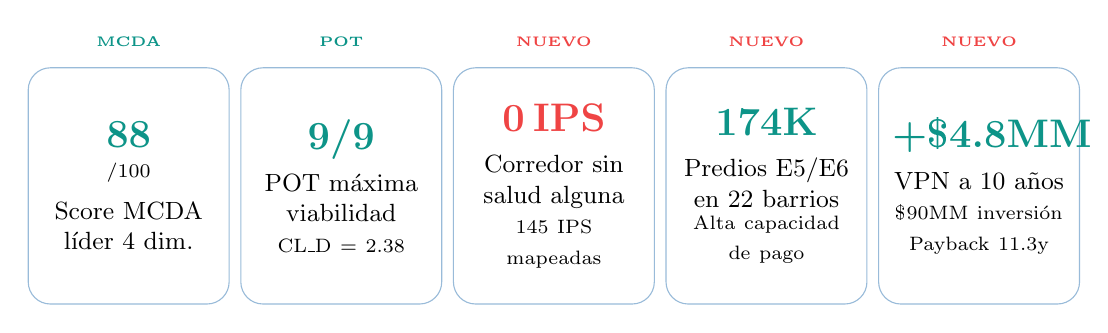
\begin{tikzpicture}[
  pillar/.style={draw=hptu!40, fill=white, rounded corners=8pt,
                 text width=2.2cm, minimum height=3.0cm, align=center,
                 font=\small, inner sep=5pt},
  plabel/.style={font=\tiny\bfseries, teal},
  newlabel/.style={font=\tiny\bfseries, coral},
]
\node[pillar] (p1) at (0,0) {
  {\Large\textcolor{teal}{\textbf{88}}}\\{\scriptsize /100}\\[4pt]
  Score MCDA\\líder 4 dim.
};
\node[pillar] (p2) at (2.7,0) {
  {\Large\textcolor{teal}{\textbf{9/9}}}\\[4pt]
  POT máxima\\viabilidad\\{\scriptsize CL\_D = 2.38}
};
\node[pillar] (p3) at (5.4,0) {
  {\Large\textcolor{coral}{\textbf{0 IPS}}}\\[4pt]
  Corredor sin\\salud alguna\\{\scriptsize 145 IPS mapeadas}
};
\node[pillar] (p4) at (8.1,0) {
  {\Large\textcolor{teal}{\textbf{174K}}}\\[4pt]
  Predios E5/E6\\en 22 barrios\\{\scriptsize Alta capacidad\\de pago}
};
\node[pillar] (p5) at (10.8,0) {
  {\Large\textcolor{teal}{\textbf{+\$4.8MM}}}\\[4pt]
  VPN a 10 años\\{\scriptsize \$90MM inversión}\\{\scriptsize Payback 11.3y}
};

\node[plabel, above=4pt of p1] {MCDA};
\node[plabel, above=4pt of p2] {POT};
\node[newlabel, above=4pt of p3] {NUEVO};
\node[newlabel, above=4pt of p4] {NUEVO};
\node[newlabel, above=4pt of p5] {NUEVO};
\end{tikzpicture}

\vspace{12pt}
\begin{columns}[T]
\column{0.48\textwidth}
\begin{exampleblock}{\small Lo que ya teníamos (Reunión 1)}
\small Score MCDA, tiempos de viaje, déficit DENSURBAM, tráfico MEData, viabilidad POT.\\[2pt]
Eso no cambió. \textbf{Se consolidó.}
\end{exampleblock}

\column{0.48\textwidth}
\begin{block}{\small Lo nuevo (Reunión 2)}
\small Red de 145 IPS confirma el vacío. Catastro cuantifica el mercado. POT completo ratifica.\\[2pt]
Y ahora sabemos que \textbf{es financieramente viable} (VPN positivo).
\end{block}
\end{columns}
\end{frame}
}

% ============================================================
% RUTA CRÍTICA: PRÓXIMOS PASOS
% ============================================================
\begin{frame}{Próximos pasos: Fase 3 — Profundización}

\begin{columns}[T]
\column{0.55\textwidth}
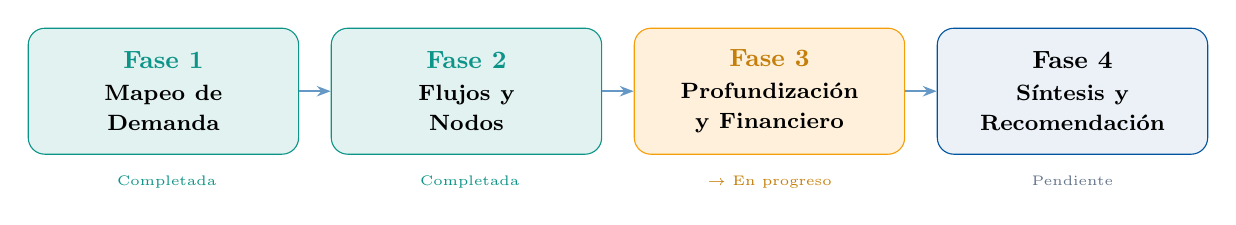
\begin{tikzpicture}[
  node distance=0.4cm,
  phase/.style={draw=hptu, fill=hptu!8, rounded corners=6pt,
                text width=3.2cm, minimum height=1.6cm, align=center,
                font=\small\bfseries},
  done/.style={phase, fill=teal!12, draw=teal},
  active/.style={phase, fill=amber!15, draw=amber},
  arrow/.style={-{Stealth[length=5pt]}, thick, hptu!60}
]
\node[done] (p1) {\textcolor{teal}{Fase 1}\\[2pt]\footnotesize Mapeo de\\Demanda};
\node[done, right=of p1] (p2) {\textcolor{teal}{Fase 2}\\[2pt]\footnotesize Flujos y\\Nodos};
\node[active, right=of p2] (p3) {\textcolor{amber!80!black}{Fase 3}\\[2pt]\footnotesize Profundización\\y Financiero};
\node[phase, right=of p3] (p4) {Fase 4\\[2pt]\footnotesize Síntesis y\\Recomendación};

\draw[arrow] (p1) -- (p2);
\draw[arrow] (p2) -- (p3);
\draw[arrow] (p3) -- (p4);

\node[below=4pt of p1, font=\tiny\color{teal}] {\checkmark\ Completada};
\node[below=4pt of p2, font=\tiny\color{teal}] {\checkmark\ Completada};
\node[below=4pt of p3, font=\tiny\color{amber!80!black}] {$\rightarrow$ En progreso};
\node[below=4pt of p4, font=\tiny\color{slate}] {Pendiente};
\end{tikzpicture}

\vspace{8pt}
\textbf{Fase 3 incluye:}
\begin{enumerate}\footnotesize
  \item Validar los 8 parámetros financieros
  \item Obtener fichas normativas POT por polígono
  \item Identificar lotes específicos disponibles
  \item Análisis competitivo detallado
  \item Modelo de demanda por especialidad
\end{enumerate}

\column{0.42\textwidth}
\begin{alertblock}{\small Lo que necesitamos}
\small
\begin{itemize}\footnotesize
  \item[\textcolor{coral}{$\blacktriangledown$}] Consulta a \textbf{Lonja de Propiedad Raíz} (precios reales suelo)
  \item[\textcolor{coral}{$\blacktriangledown$}] Estados financieros de \textbf{hospitales comparables}
  \item[\textcolor{coral}{$\blacktriangledown$}] Fichas normativas \textbf{DAP Medellín}
  \item[\textcolor{amber}{$\blacktriangledown$}] Acceso a \textbf{Supersalud} (márgenes operativos)
  \item[\textcolor{amber}{$\blacktriangledown$}] Contacto con \textbf{inmobiliarias} del corredor
\end{itemize}
\end{alertblock}

\vspace{6pt}
\begin{block}{\small Entregables Fase 3}
\small
\begin{enumerate}\footnotesize
  \item Modelo financiero validado
  \item Shortlist de 2--3 lotes específicos
  \item Due diligence normativa (POT + EIA)
  \item Análisis de sensibilidad robusto
\end{enumerate}
\end{block}
\end{columns}
\end{frame}

% ============================================================
% RESUMEN EJECUTIVO
% ============================================================
\begin{frame}{Resumen ejecutivo}

\begin{columns}[T]
\column{0.55\textwidth}
\begin{block}{\small Lo que confirmamos hoy}
\footnotesize
\begin{enumerate}
  \item Corredor Las Palmas: \highlight{0 IPS} (145 puntos mapeados)
  \item Mercado: \highlight{174,543 predios} E5/E6 en 22 barrios
  \item POT: uso dotacional salud con \highlight{score 9/9}
  \item Financiero: \highlight{VPN positivo} en 4 de 5 zonas
  \item Las Palmas Bajo: \highlight{mejor balance} integral
\end{enumerate}
\end{block}

\column{0.42\textwidth}
\begin{alertblock}{\small Lo que falta para decidir}
\footnotesize
\begin{enumerate}
  \item Validar supuestos financieros con el sector
  \item Fichas normativas POT por polígono
  \item Lotes disponibles con propietarios
  \item Análisis de sensibilidad completo
  \item Escenarios para la Junta
\end{enumerate}
\end{alertblock}

\vspace{4pt}
{\footnotesize\textcolor{slate}{La recomendación se sostiene con más fuerza, pero necesitamos validar los números antes de una decisión de \textbf{\$90+ mil millones COP}.}}
\end{columns}
\end{frame}

% ============================================================
% CIERRE
% ============================================================
{
\setbeamercolor{background canvas}{bg=hptu}
\begin{frame}[plain]
\vfill
\begin{center}
{\Huge\bfseries\textcolor{white}{¿Preguntas?}}

\vspace{20pt}
\begin{tikzpicture}
  \draw[white, line width=0.5pt] (0,0) -- (6,0);
\end{tikzpicture}

\vspace{16pt}
{\large\textcolor{white!90}{HPTU — Estudio de Localización Estratégica}}

\vspace{10pt}
{\small\textcolor{white!70}{Plataforma: \url{https://hptu-localizacion.vercel.app}}}

\vspace{6pt}
{\small\textcolor{white!70}{12 capas interactivas $\cdot$ 145 IPS $\cdot$ Modelo financiero preliminar}}

\vspace{6pt}
{\small\textcolor{white!60}{Segunda reunión de avance — 4 de marzo, 2026}}

\vspace{20pt}
{\footnotesize\textcolor{white!40}{Todo es datos. Nada es opinión.}}
\end{center}
\vfill
\end{frame}
}

\end{document}
